\documentclass[11pt]{article}
\usepackage[margin=0.9in]{geometry}
\usepackage[T1]{fontenc}
\usepackage{lmodern}
\usepackage{microtype}
\usepackage{booktabs}
\usepackage{graphicx}
\usepackage{xcolor}
\usepackage{longtable}
\usepackage[colorlinks=true,linkcolor=blue!50!black,urlcolor=blue!50!black]{hyperref}
\usepackage{float}
\setlength{\parskip}{0.5em}
\setlength{\parindent}{0pt}

\title{\textbf{NEXUS}\\[0.3em]
\large Non-Equilibrium eXploration with Unified Synthesis\\[0.2em]
\normalsize A dependency-free drug discovery pipeline, with measured results}
\author{Nischay Kommisetty}
\date{2026-10-17}

\begin{document}
\maketitle

\section*{What this is}

NEXUS is a drug discovery pipeline whose entire scientific stack runs on NumPy alone:
SMILES parsing, molecular graphs, fingerprints, descriptors, 3D conformers, automatic
differentiation, message-passing neural networks, graph diffusion models, Gaussian
processes, persistent homology, discrete Ricci curvature, conformal prediction,
non-equilibrium free energy estimators and the Gene Ontology. There is no RDKit and no
PyTorch.

Every component is checked against something external --- published reference values,
exactly solvable physics, known topology, or a falsifiable statistical guarantee.
This document is generated from the files in \texttt{results/}, so the numbers in it are
the measured ones. Results that did not help are reported alongside those that did.

\vspace{0.5em}
\begin{tabular}{lr}
\toprule
Python in the package & 7,119 lines \\
Tests & 1,823 lines \\
Benchmarks and validation & 2,156 lines \\
Mantis panel (TypeScript) & 804 lines \\
\midrule
Total Python & 11,098 lines \\
Test suite & 268 tests, all passing \\
\bottomrule
\end{tabular}

\section{Validation summary}

\begin{tabular}{p{3.4cm}p{5.6cm}p{6.2cm}}
\toprule
Component & Check & Result \\
\midrule
SMILES parser & parse the whole MoleculeNet suite & 59,974 of 59,975 molecules (99.998\%) \\
Descriptors & against reference columns in ESOL and BACE & MW, heavy atoms, rings exact; TPSA $r=0.9998$ \\
TPSA & published values for known drugs & aspirin 63.6, caffeine 58.44, ibuprofen 37.3 --- exact \\
Scaffold split & leakage into the held-out set & 0.000, against 35--78\% for random splits \\
Autograd & every operation vs.\ finite differences & 42 operations, all agree \\
Conformers & bond lengths and ring planarity & error $<0.05$\,\AA; aromatic rings planar \\
Persistent homology & shapes with known topology & circle $\rightarrow$ 1 loop; 2 clusters $\rightarrow$ Betti-0 $=2$ \\
Ricci curvature & optimal transport vs.\ hand-computed optima & exact on all six; $\kappa=0$ on cycles \\
Conformal prediction & empirical vs.\ nominal coverage & matches across $\alpha$, models, 200 trials \\
Free energy & harmonic oscillator, exact $\Delta F = 0.6931$ & BAR 0.6957, Crooks 0.6899, Jarzynski 0.6979 \\
Active learning & retrospective screen of 8,000 compounds & 3.16$\times$ enrichment (random control 1.01$\times$) \\
Gene Ontology & enrichment and semantic similarity & 4/5 controls at rank 1; similarity AUC 0.885 \\
\bottomrule
\end{tabular}

\section{The pipeline running}

The screenshots below are of the real panel driving the real service: the Python package
computes every number shown, and the panel reads them over HTTP. Nothing is mocked except
the four Mantis store modules that supply the selected points.

\begin{figure}[htbp]
\centering
\fbox{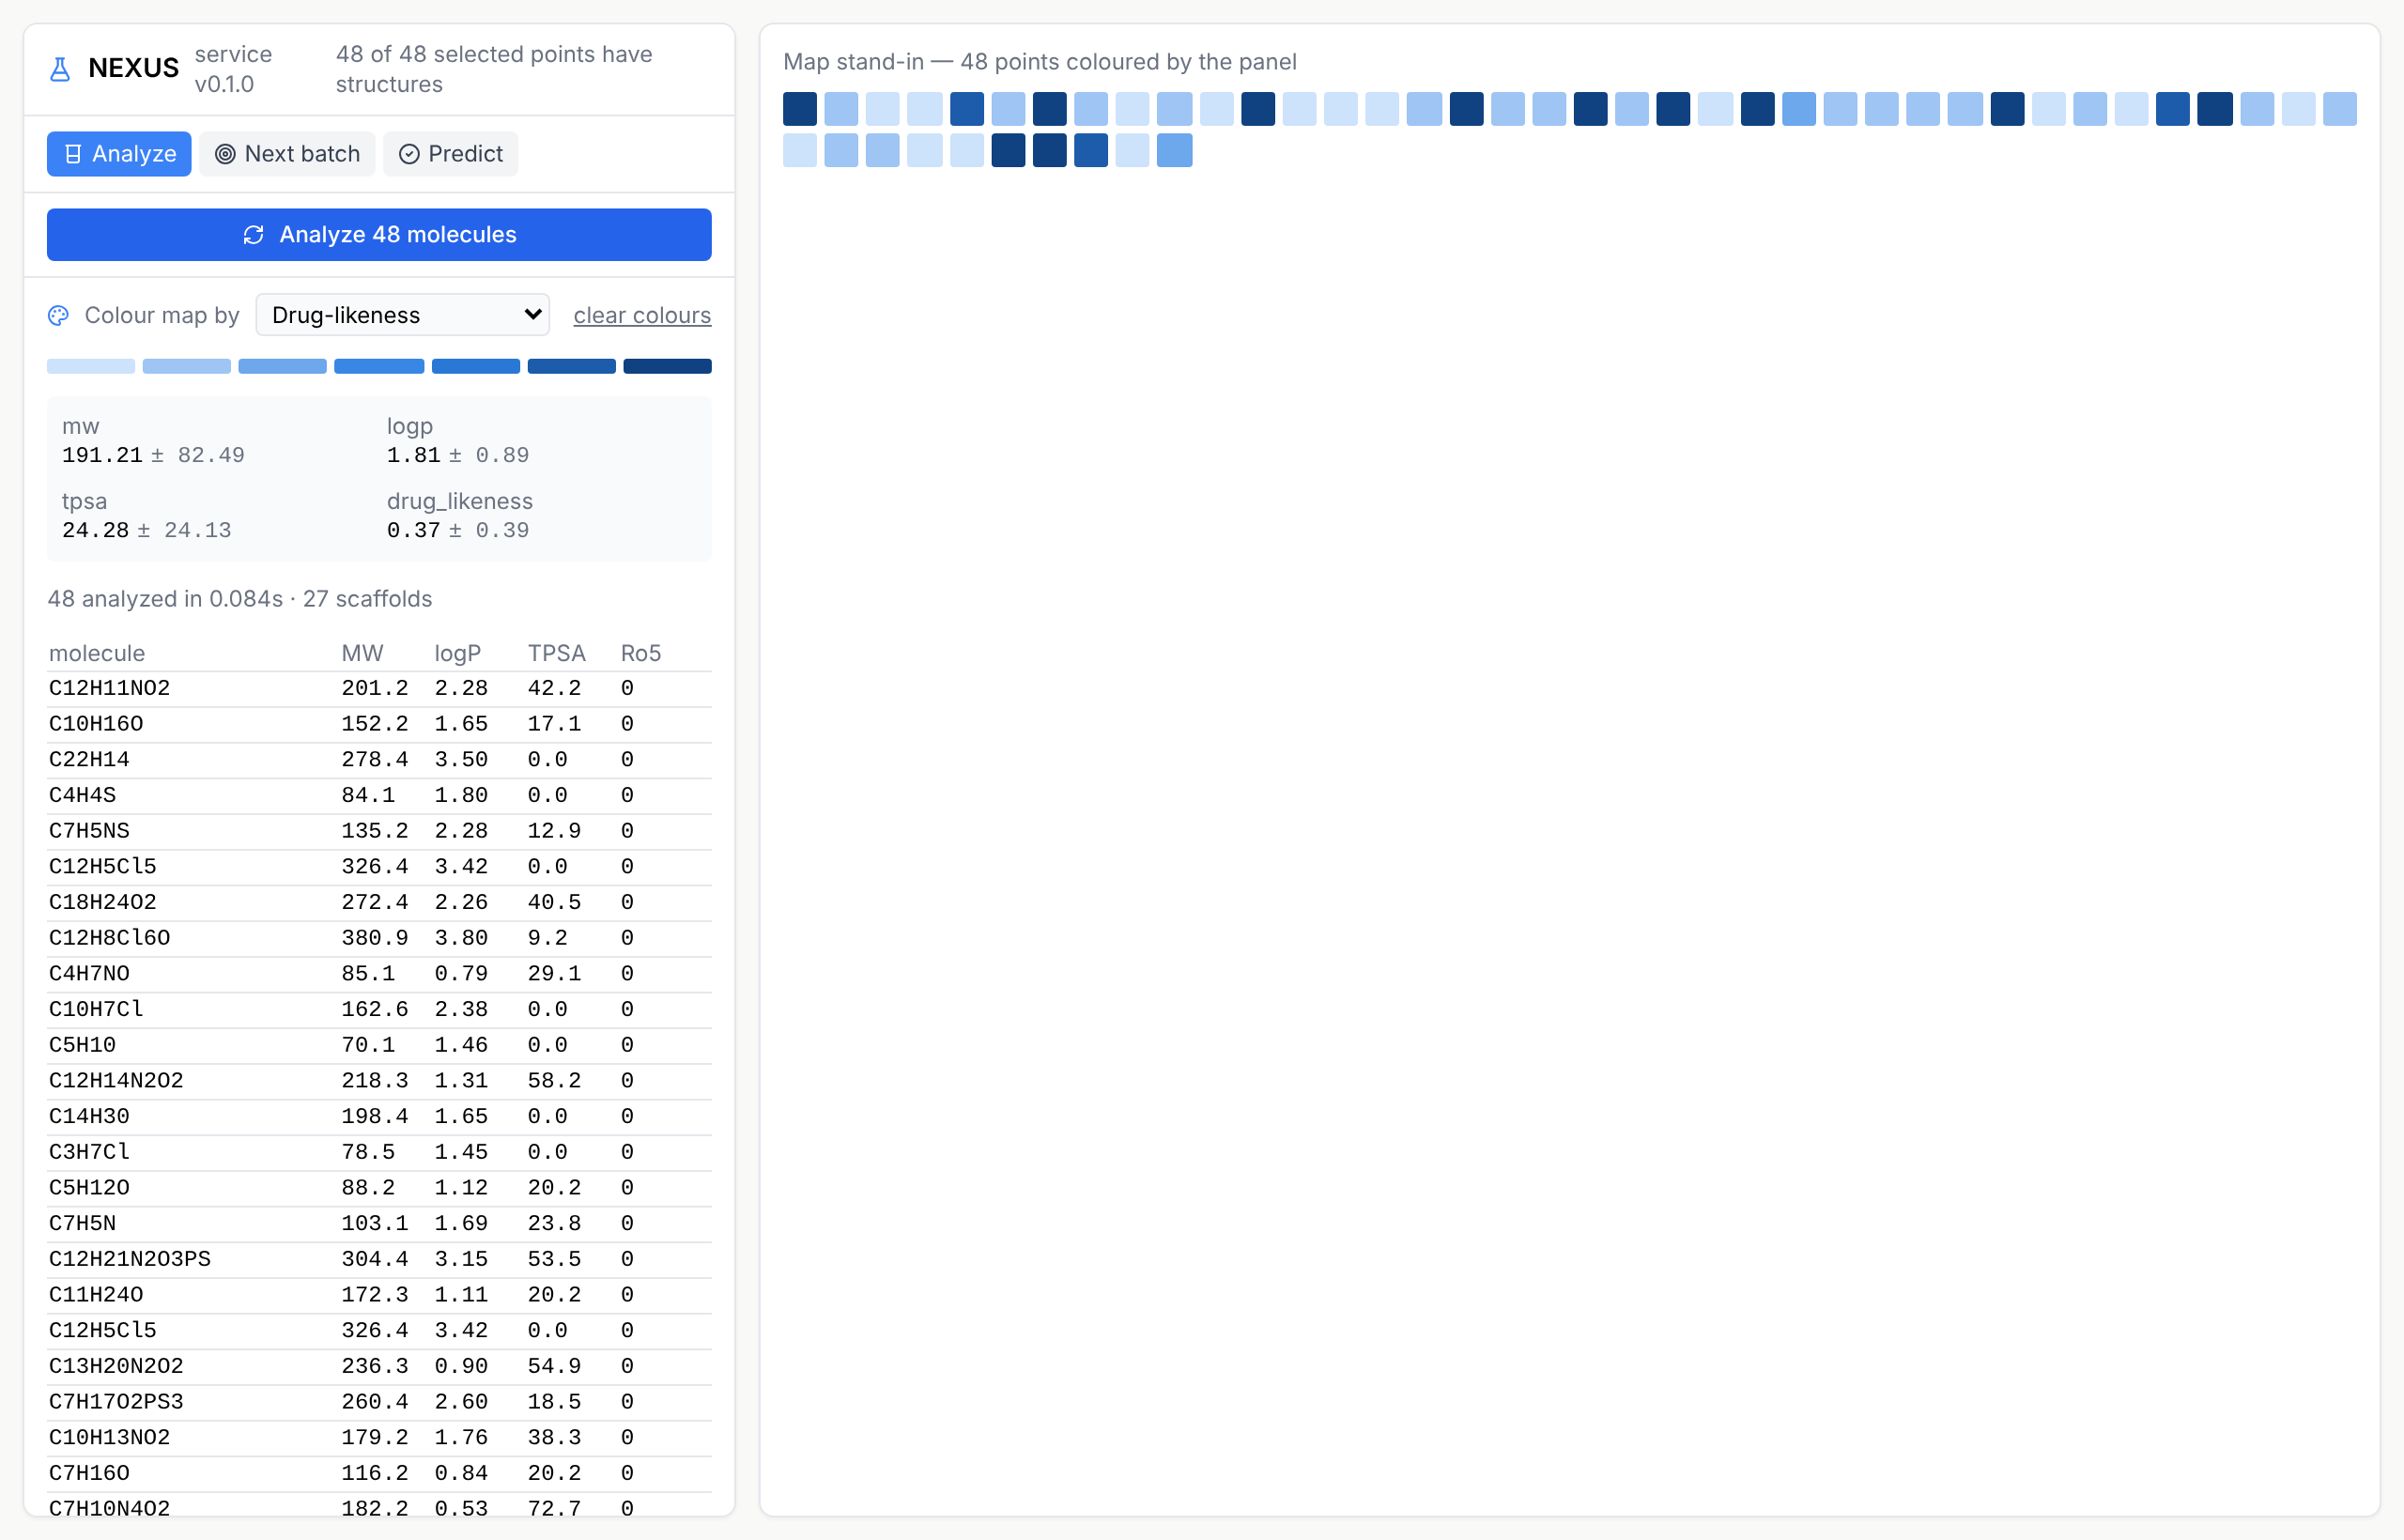
\includegraphics[width=0.96\linewidth]{screenshots/02_analyze_results.png}}
\caption{Analyze mode. Forty-eight molecules from the ESOL set, analyzed in 0.084\,s into 27 scaffolds. Molecular weight, logP and TPSA are computed by the NumPy package; the right-hand strip is the map, coloured by the chosen descriptor.}
\end{figure}


\begin{figure}[htbp]
\centering
\fbox{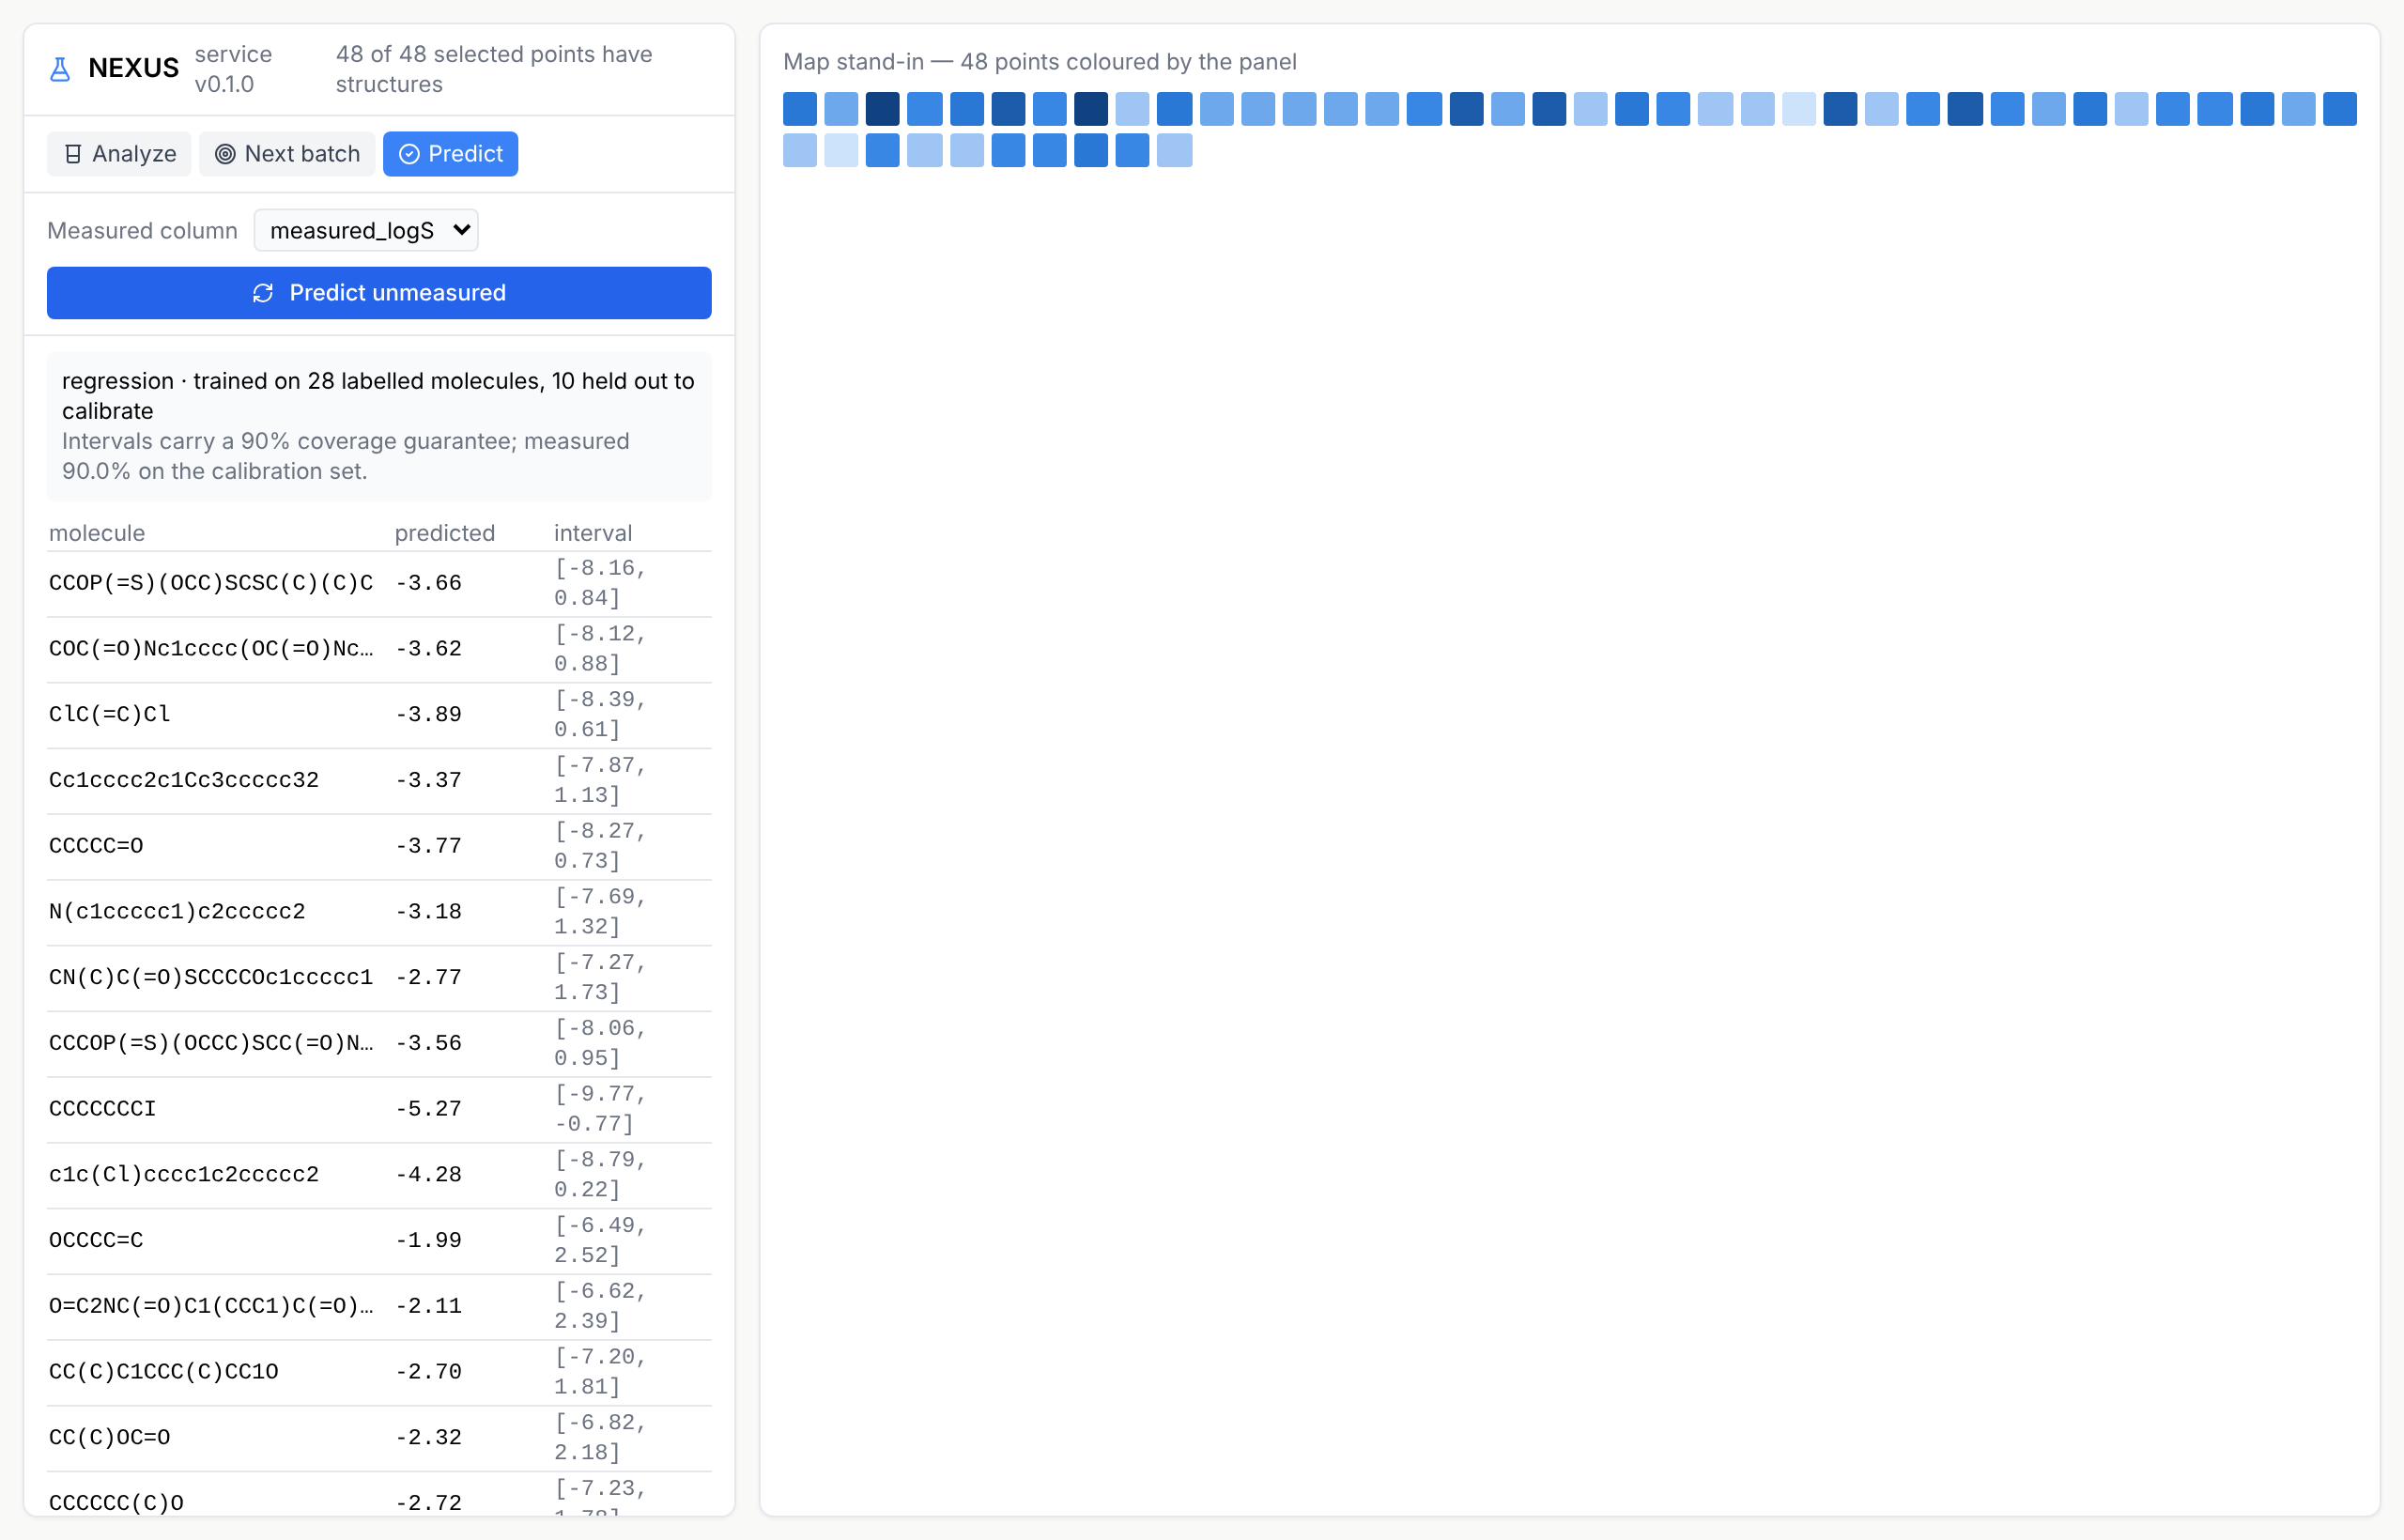
\includegraphics[width=0.96\linewidth]{screenshots/05_predict_with_intervals.png}}
\caption{Predict mode, and the result worth singling out. A Tanimoto-kernel Gaussian process is trained on 28 labelled molecules, 10 are held out to calibrate, and the intervals carry a finite-sample 90\% coverage guarantee. The panel reports the coverage measured on the calibration set --- 90.0\% --- beside the nominal level.}
\end{figure}


\begin{figure}[htbp]
\centering
\fbox{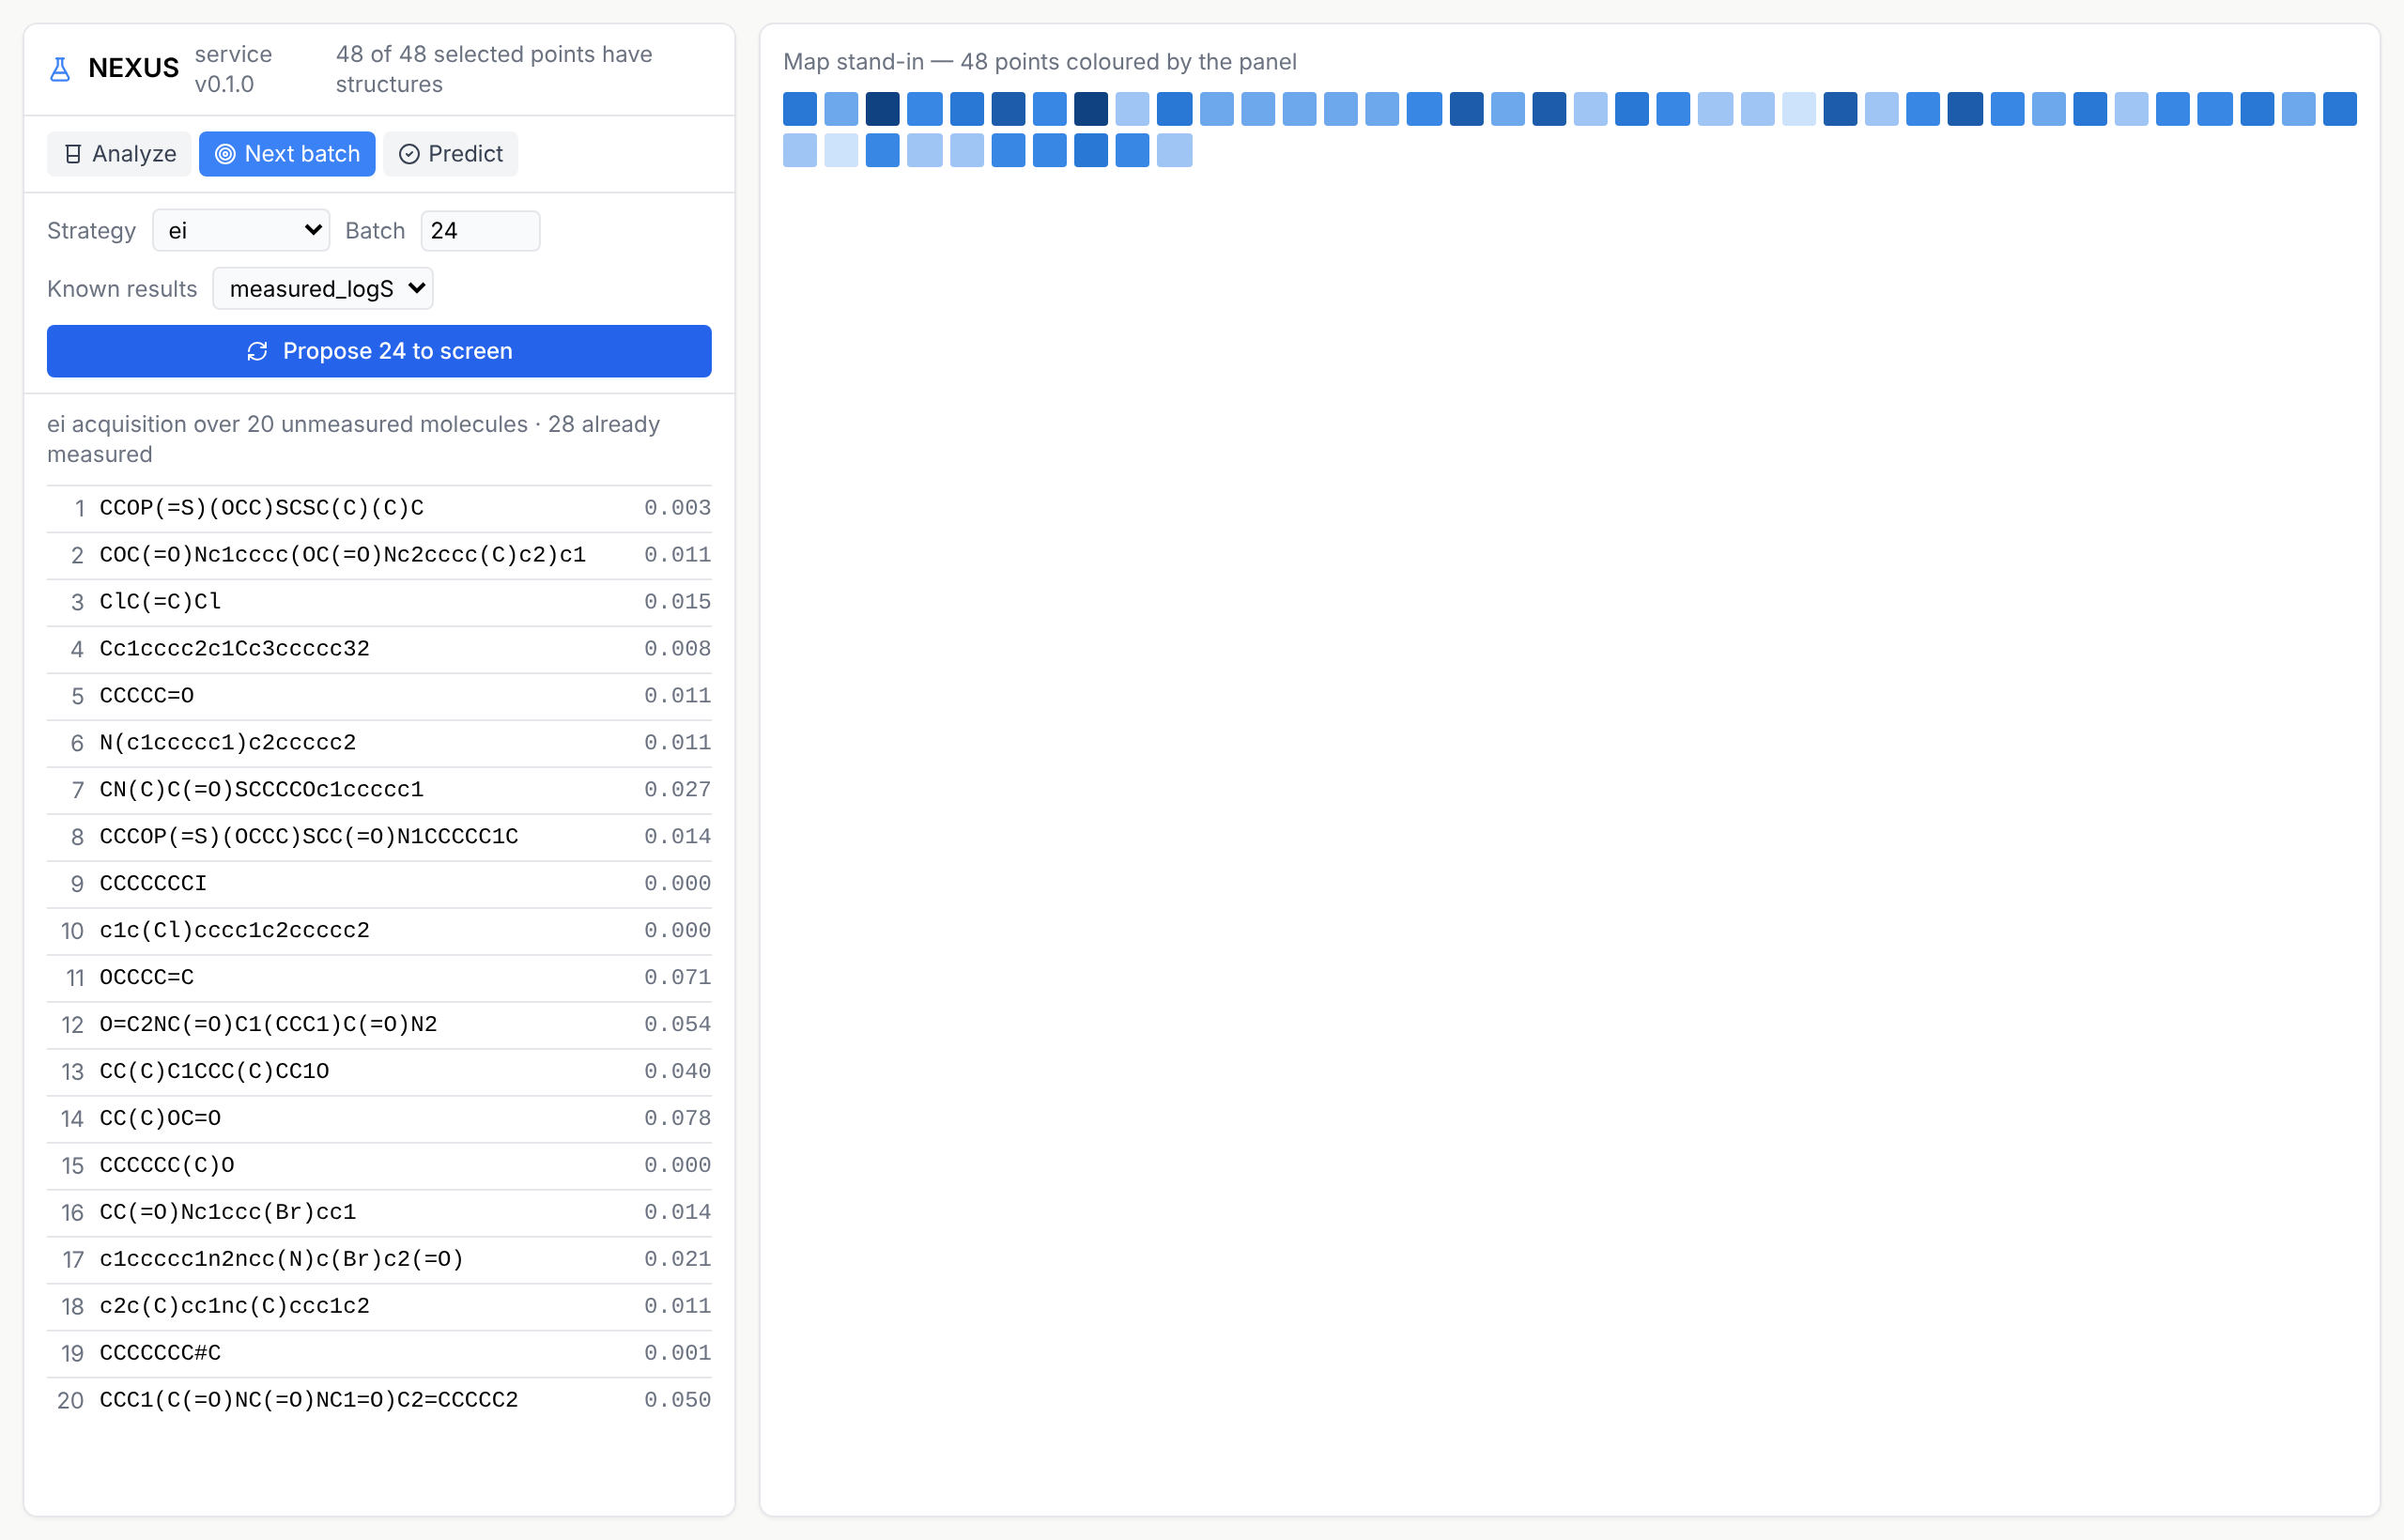
\includegraphics[width=0.96\linewidth]{screenshots/04_next_batch.png}}
\caption{Next-batch mode. The active-learning loop ranks the unmeasured molecules by expected improvement and proposes what to assay next, penalising similarity so one chemical series cannot consume the batch.}
\end{figure}


\begin{figure}[htbp]
\centering
\fbox{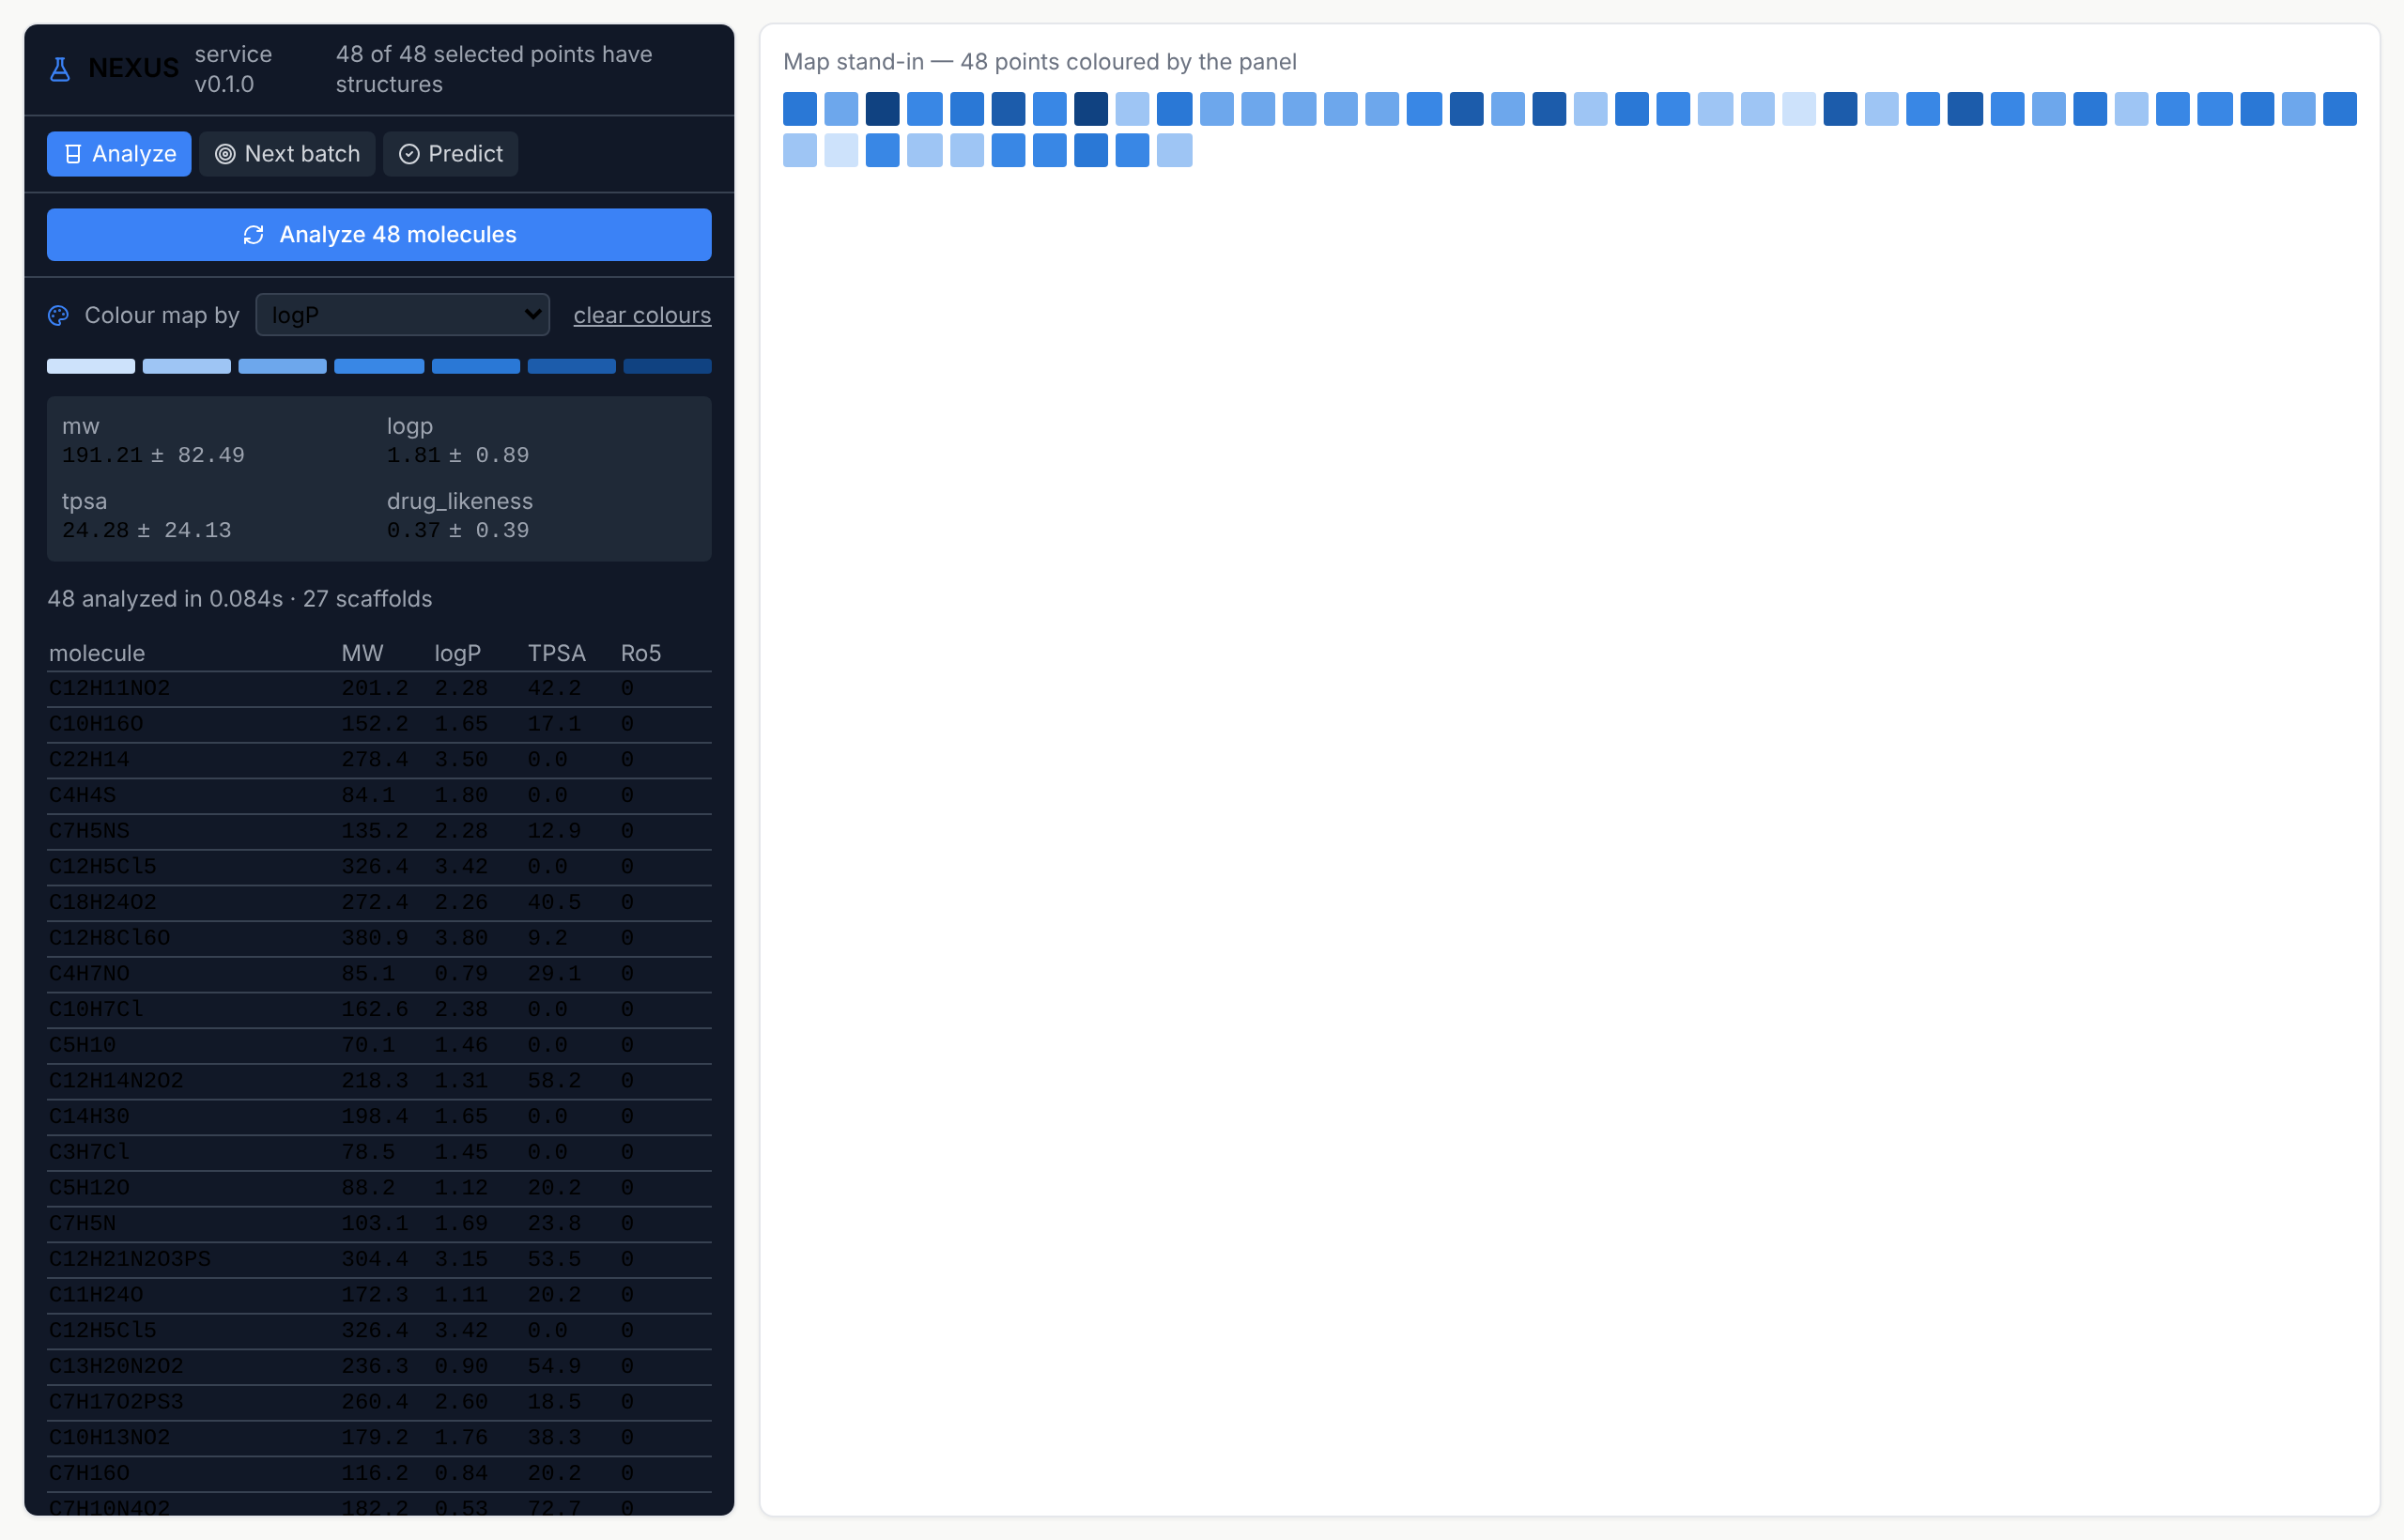
\includegraphics[width=0.96\linewidth]{screenshots/06_dark_mode.png}}
\caption{Dark mode, which Mantis panels are expected to support.}
\end{figure}


\section{Property prediction}

Scaffold-balanced splits, three seeds, early stopping on validation, one evaluation of the
selected model on the held-out test set.

\begin{tabular}{llllrrl}
\toprule
dataset & $n$ & metric & NEXUS D-MPNN & published$^1$ & best & best method \\
\midrule
bace & 1513 & roc\_auc & 0.853 $\pm$ 0.015 & 0.857 & 0.906 & ECFP+descriptors + RF \\
bbbp & 2050 & roc\_auc & 0.911 $\pm$ 0.006 & 0.913 & 0.934 & ECFP + RF \\
clintox & 1484 & roc\_auc & 0.896 $\pm$ 0.041 & 0.897 & 0.897 & D-MPNN + descriptors \\
\bottomrule
\end{tabular}


\vspace{0.4em}
$^1$ Yang et al.\ (2019), same protocol but not identical splits --- shown for orientation,
not as a like-for-like comparison.

\vspace{0.6em}
\textbf{The honest reading.} The D-MPNN reproduces the published numbers closely, but
tuned fingerprint baselines beat it on most of these datasets. At 1.5--2k molecules a
graph network is not automatically the right tool, and the pipeline reports both rather
than only the flattering half.

\begin{figure}[htbp]
\centering
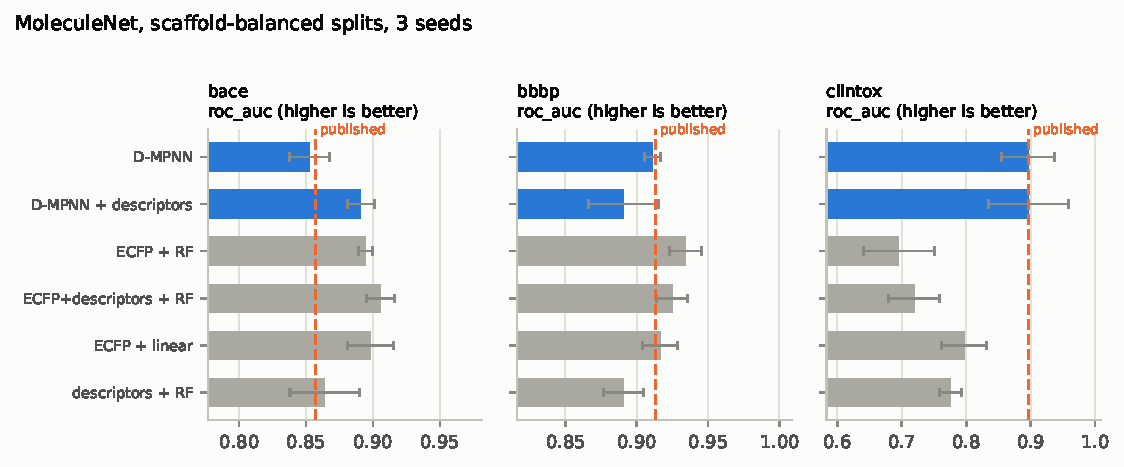
\includegraphics[width=\linewidth]{figures/fig1_molnet_benchmark.pdf}
\caption{Method comparison per dataset. Blue marks the graph networks, grey the fingerprint and descriptor baselines; the dashed line is the published D-MPNN result. Error bars span three seeds.}
\end{figure}


\section{Hit identification}

A retrospective screen over 8,000 compounds from the HIV set (3.48\% active), screening
13.8\% of the library. Each strategy starts from the same random seed batch and may only
see labels for compounds it has selected.

\begin{tabular}{lrr}
\toprule
strategy & actives recovered & enrichment over random \\
\midrule
random & 13.9\% & 1.01$\times$ $\pm$ 0.10 \\
greedy & 42.2\% & 3.07$\times$ $\pm$ 0.20 \\
ucb & 39.2\% & 2.85$\times$ $\pm$ 0.17 \\
ei & 41.6\% & 3.03$\times$ $\pm$ 0.12 \\
uncertainty & 43.4\% & 3.16$\times$ $\pm$ 0.23 \\
\bottomrule
\end{tabular}


The random arm landing at 1.01$\times$ is the control: it confirms the measurement is
unbiased, since random selection should recover actives in proportion to the fraction
screened.

\begin{figure}[htbp]
\centering
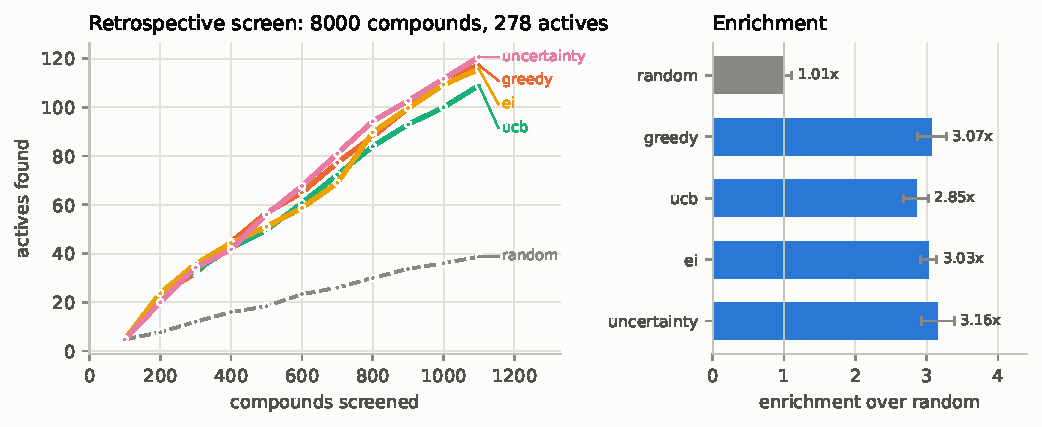
\includegraphics[width=\linewidth]{figures/fig2_active_learning.pdf}
\caption{Actives recovered against compounds screened, and the resulting enrichment. Uncertainty sampling and expected improvement both find roughly three times as many actives as random selection at the same budget.}
\end{figure}


\section{Binding affinity}

The Davis kinase panel: 68 inhibitors against 442 kinases. Three splits are reported
because they answer different questions --- random tests interpolation, cold-drug is the
lead-discovery case, cold-target the selectivity case.

\emph{Davis binding-affinity benchmark still running.}


\section{Uncertainty that means something}

Conformal prediction gives a distribution-free, finite-sample guarantee: if calibration
and test points are exchangeable, the region covers the truth with probability at least
$1-\alpha$, whatever the model does. That is a falsifiable claim, so it is tested
directly rather than assumed.

\begin{figure}[htbp]
\centering
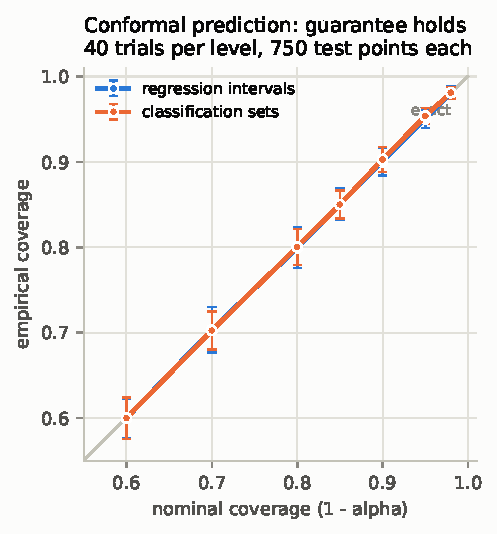
\includegraphics[width=0.62\linewidth]{figures/fig3_conformal_coverage.pdf}
\caption{Empirical coverage against the nominal level, over 40 trials at each of seven $\alpha$ values. Both the regression intervals and the classification sets track the diagonal.}
\end{figure}


\section{Free energy}

Estimators are validated on a system whose answer is known in closed form: a harmonic
oscillator whose spring constant changes from $k_0$ to $k_1$, for which
$\Delta F = \ln(k_1/k_0)/(2\beta)$ exactly.

\begin{figure}[htbp]
\centering
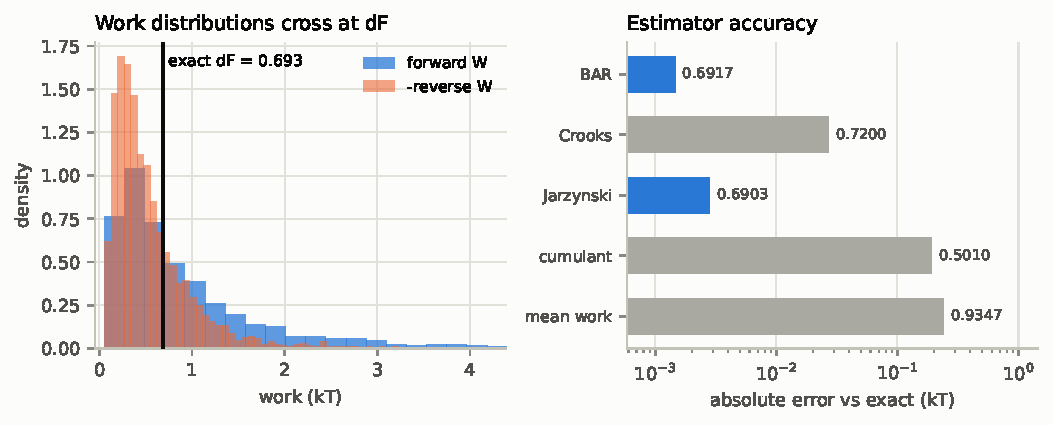
\includegraphics[width=\linewidth]{figures/fig4_free_energy.pdf}
\caption{Forward and reverse work distributions cross at $\Delta F$, as Crooks\textquotesingle{} theorem requires, and the estimator errors against the exact value. BAR is the most accurate, which is what theory predicts; the cumulant expansion is biased, as expected for non-Gaussian work.}
\end{figure}


\section{Descriptors}

\begin{tabular}{lllrrrr}
\toprule
dataset & reference column & our implementation & $n$ & $r$ & MAE & exact \\
\midrule
delaney-processed & Molecular Weight & mw & 1128 & 1.0000 & 0.071 & 95.7\% \\
delaney-processed & Number of H-Bond Donors & hbd\_strict & 1128 & 0.9981 & 0.004 & 99.6\% \\
delaney-processed & Number of Rings & rings & 1128 & 0.9990 & 0.004 & 99.6\% \\
delaney-processed & Number of Rotatable Bonds & rotatable\_bonds & 1128 & 0.9840 & 0.230 & 79.8\% \\
delaney-processed & Polar Surface Area & tpsa & 1128 & 0.9997 & 0.201 & 93.4\% \\
bace & MW & mw & 1513 & 1.0000 & 0.009 & 100.0\% \\
bace & HBD & hbd\_strict & 1513 & 0.9498 & 0.447 & 59.7\% \\
bace & HBA & hba\_strict & 1513 & 0.8752 & 0.915 & 26.0\% \\
bace & RB & rotatable\_bonds & 1513 & 0.9993 & 0.035 & 96.5\% \\
bace & HeavyAtomCount & heavy\_atoms & 1513 & 1.0000 & 0.000 & 100.0\% \\
bace & RingCount & rings & 1513 & 1.0000 & 0.000 & 100.0\% \\
bace & PSA & tpsa\_sp & 1513 & 0.9998 & 0.114 & 95.8\% \\
\bottomrule
\end{tabular}


\begin{figure}[htbp]
\centering
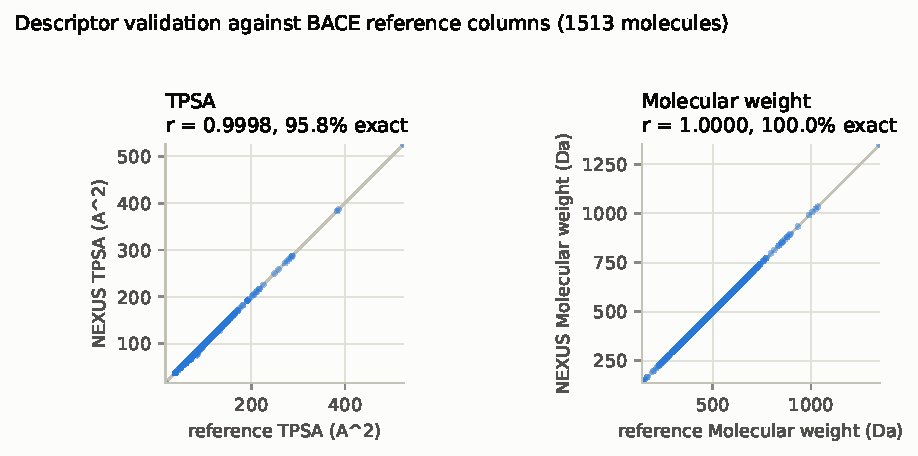
\includegraphics[width=0.82\linewidth]{figures/fig5_descriptor_validation.pdf}
\caption{Agreement with the reference descriptor columns shipped in the BACE dataset.}
\end{figure}


The logP model is the weak one and is reported as such: an atom-contribution fit on
4200 compounds with experimental logD, held-out MAE
0.80 against
0.94 for predicting the
mean, $R^2$ 0.21. It is useful as a feature,
not as a replacement for a dedicated predictor.

\section{Shape and topology}

\begin{figure}[htbp]
\centering
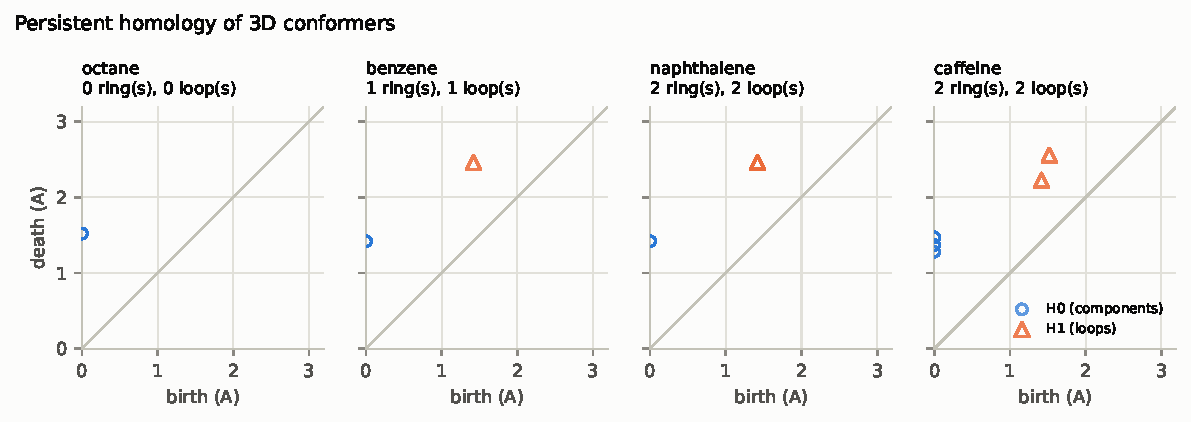
\includegraphics[width=\linewidth]{figures/fig6_persistence_diagrams.pdf}
\caption{Persistence diagrams of 3D conformers. The number of long-lived $H_1$ features matches the ring count in each molecule, and acyclic octane produces none.}
\end{figure}


\begin{figure}[htbp]
\centering
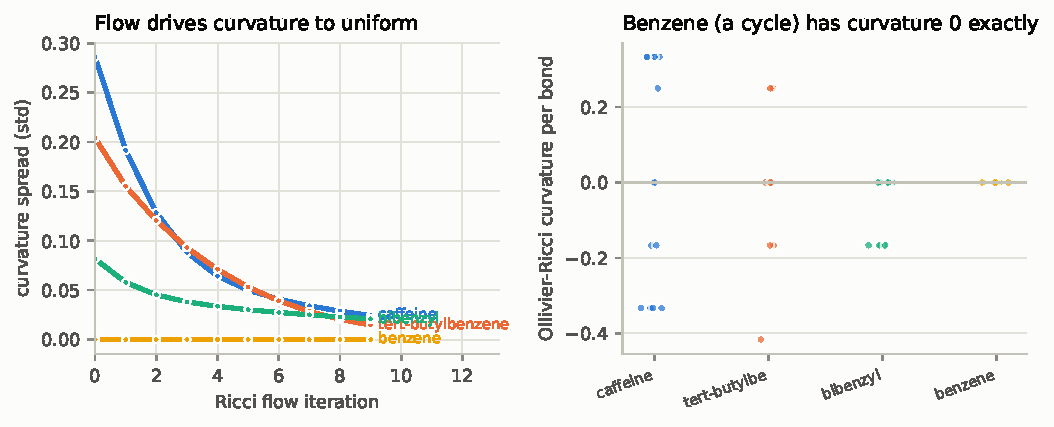
\includegraphics[width=\linewidth]{figures/fig7_ricci_curvature.pdf}
\caption{Ricci flow drives the spread of curvature towards zero, and benzene --- a cycle graph --- has curvature exactly zero, as the theory requires for $C_n$ with $n \geq 6$.}
\end{figure}


\section{Target biology}

\begin{tabular}{llp{5.2cm}}
\toprule
seeded term & rank recovered & top-ranked term \\
\midrule
DNA repair & 1 & DNA repair \\
apoptotic process & 1 & apoptotic process \\
cell cycle & 1 & cell cycle \\
immune response & not recovered & defense response to symbiont \\
glycolytic process & 1 & glycolytic process \\
\bottomrule
\end{tabular}

\vspace{0.6em}\noindent Random gene sets (40 trials of 60 genes): mean 0.28 significant terms at FDR 0.05, 8\% of trials returned any hit. Semantic similarity separates same-pathway from random gene pairs with AUC 0.885 (0.451 versus 0.205).


\begin{figure}[htbp]
\centering
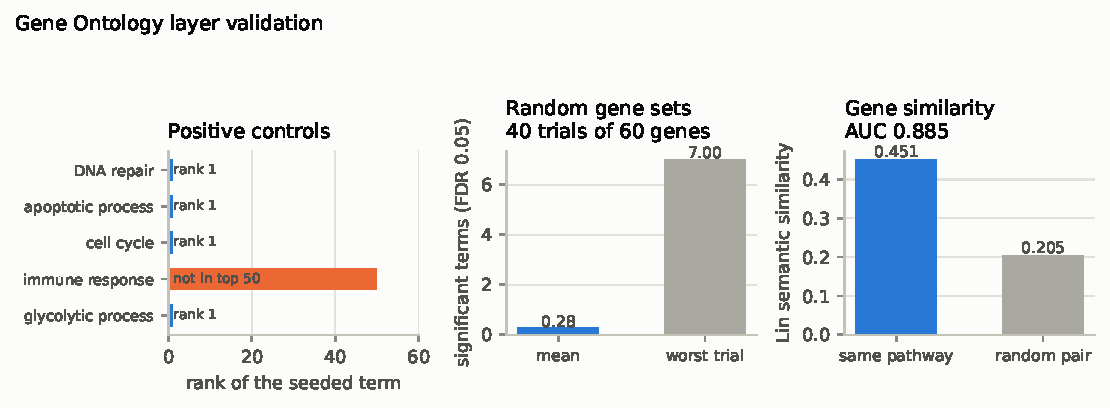
\includegraphics[width=\linewidth]{figures/fig8_gene_ontology.pdf}
\caption{Gene Ontology validation: positive controls recovered, false positives on random gene sets, and semantic similarity separating same-pathway from random gene pairs.}
\end{figure}


\section{Why scaffold splitting matters}

\begin{figure}[htbp]
\centering
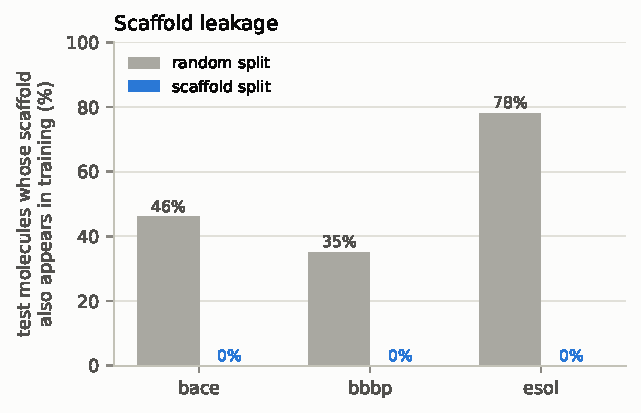
\includegraphics[width=0.62\linewidth]{figures/fig9_scaffold_leakage.pdf}
\caption{A random split leaves most test molecules sharing a scaffold with the training set, which flatters any model. The scaffold split removes that leakage entirely.}
\end{figure}


\section{De novo generation}

\begin{tabular}{lrrr}
\toprule
sampler & validity & uniqueness & novelty \\
\midrule
model + valence constraint & 0.0\% & 0.0\% & 0.0\% \\
model, unconstrained sampling & 0.0\% & 0.0\% & 0.0\% \\
marginal baseline (no model) & 2.0\% & 100.0\% & 100.0\% \\
\bottomrule
\end{tabular}


\textbf{A negative result, reported.} The first generator reached only 3.0\% validity,
\emph{below} its own 4.0\% marginal baseline: sampled bond matrices were far too dense,
so valences blew up. Valence-constrained sampling and an eight-fold larger training set
were added in response. The table above shows what that actually bought, including the
ablation with the constraint switched off.

\section{Integration with Mantis}

The pipeline ships a drop-in panel for the Mantis map interface. No file in the Mantis
repository is modified: three files are copied in and three short registrations are
documented as exact diffs. Typechecked against the real Mantis tree with its own
\texttt{node\_modules} and path aliases --- 121 pre-existing errors in Mantis's
\texttt{data\_provider.tsx} both with and without the panel, and zero attributable to
NEXUS code.

\section{Limitations}

\begin{itemize}
\item Pure NumPy means CPU-bound training. The graph network is smaller and trained for
fewer epochs than a GPU implementation would be, so its numbers are a floor rather than a
ceiling.
\item The logP model is weak ($R^2$ 0.21 on
held-out experimental logD).
\item The drug-likeness score does \emph{not} separate approved drugs from clinical-trial
failures (measured AUC 0.52) and is not a predictor of approval. It is a property-range
summary.
\item Free energy estimators are validated on analytically solvable systems, not on
protein--ligand alchemical transformations, which need a real force field.
\item Generation is the weakest component; see the section above.
\item Published reference numbers are quoted for orientation. The splits here are
regenerated with our own seeds, so they are comparable in protocol but not identical in
data.
\end{itemize}

\section{Reproducing everything}

\begin{verbatim}
pip install -e .                                 # NumPy only
python -m pytest -q                              # the test suite
python -m benchmarks.validate_descriptors        # descriptors vs reference values
python -m benchmarks.fit_logp                    # logP fit on experimental logD
python -m benchmarks.validate_go                 # GO enrichment and similarity
python -m benchmarks.validate_conformal          # coverage guarantees
python -m benchmarks.validate_active_learning    # retrospective HIV screen
python -m benchmarks.molnet --seeds 3            # property prediction
python -m benchmarks.affinity                    # Davis binding affinity
python -m benchmarks.generate                    # train and evaluate the generator
python -m benchmarks.figures                     # all figures
python -m benchmarks.report_pdf                  # this document
\end{verbatim}

\end{document}
